\documentclass{book}
\usepackage[letterpaper,top=2.5cm,bottom=2.5cm,left=2.5cm,right=2.5cm]{geometry}
\usepackage{makeidx}
\usepackage{natbib}
\usepackage{graphicx}
\usepackage{multicol}
\usepackage{float}
\usepackage{listings}
\usepackage{color}
\usepackage{ifthen}
\usepackage[table]{xcolor}
\usepackage{textcomp}
\usepackage{alltt}
\usepackage{ifpdf}
\ifpdf
\usepackage[pdftex,
            pagebackref=true,
            colorlinks=true,
            linkcolor=blue,
            unicode
           ]{hyperref}
\else
\usepackage[ps2pdf,
            pagebackref=true,
            colorlinks=true,
            linkcolor=blue,
            unicode
           ]{hyperref}
\usepackage{pspicture}
\fi
\usepackage[utf8]{inputenc}
\usepackage{mathptmx}
\usepackage[scaled=.90]{helvet}
\usepackage{courier}
\usepackage{sectsty}
\usepackage{amssymb}
\usepackage[titles]{tocloft}
\usepackage{doxygen}
\lstset{language=C++,inputencoding=utf8,basicstyle=\footnotesize,breaklines=true,breakatwhitespace=true,tabsize=4,numbers=left }
\makeindex
\setcounter{tocdepth}{3}
\renewcommand{\footrulewidth}{0.4pt}
\renewcommand{\familydefault}{\sfdefault}
\hfuzz=15pt
\setlength{\emergencystretch}{15pt}
\hbadness=750
\tolerance=750
\begin{document}
\hypersetup{pageanchor=false,citecolor=blue}
\begin{titlepage}
\vspace*{7cm}
\begin{center}
{\Large Open\-Gui }\\
\vspace*{1cm}
{\large Generated by Doxygen 1.8.2}\\
\vspace*{0.5cm}
{\small Thu Nov 1 2012 01:55:19}\\
\end{center}
\end{titlepage}
\clearemptydoublepage
\pagenumbering{roman}
\tableofcontents
\clearemptydoublepage
\pagenumbering{arabic}
\hypersetup{pageanchor=true,citecolor=blue}
\chapter{Class Index}
\section{Class List}
Here are the classes, structs, unions and interfaces with brief descriptions\-:\begin{DoxyCompactList}
\item\contentsline{section}{\hyperlink{class_button}{Button} }{\pageref{class_button}}{}
\item\contentsline{section}{\hyperlink{class_check_box}{Check\-Box} }{\pageref{class_check_box}}{}
\item\contentsline{section}{\hyperlink{class_element}{Element} \\*The base class that all G\-U\-I elements derive from }{\pageref{class_element}}{}
\item\contentsline{section}{\hyperlink{class_image}{Image} }{\pageref{class_image}}{}
\item\contentsline{section}{\hyperlink{class_image_element}{Image\-Element} }{\pageref{class_image_element}}{}
\item\contentsline{section}{\hyperlink{class_pixel}{Pixel} }{\pageref{class_pixel}}{}
\item\contentsline{section}{\hyperlink{class_text}{Text} }{\pageref{class_text}}{}
\item\contentsline{section}{\hyperlink{class_text_element}{Text\-Element} }{\pageref{class_text_element}}{}
\item\contentsline{section}{\hyperlink{class_toggle_button}{Toggle\-Button} }{\pageref{class_toggle_button}}{}
\end{DoxyCompactList}

\chapter{File Index}
\section{File List}
Here is a list of all files with brief descriptions\-:\begin{DoxyCompactList}
\item\contentsline{section}{\hyperlink{main_8cpp}{main.\-cpp} }{\pageref{main_8cpp}}{}
\item\contentsline{section}{\hyperlink{main_8h}{main.\-h} }{\pageref{main_8h}}{}
\item\contentsline{section}{button/\hyperlink{_button_8h}{Button.\-h} }{\pageref{_button_8h}}{}
\item\contentsline{section}{button/\hyperlink{button_2main_8cpp}{main.\-cpp} }{\pageref{button_2main_8cpp}}{}
\item\contentsline{section}{checkbox/\hyperlink{_check_box_8h}{Check\-Box.\-h} }{\pageref{_check_box_8h}}{}
\item\contentsline{section}{element/\hyperlink{_element_8cpp}{Element.\-cpp} }{\pageref{_element_8cpp}}{}
\item\contentsline{section}{element/\hyperlink{_element_8h}{Element.\-h} }{\pageref{_element_8h}}{}
\item\contentsline{section}{element/\hyperlink{element_2main_8cpp}{Main.\-cpp} }{\pageref{element_2main_8cpp}}{}
\item\contentsline{section}{image/\hyperlink{_image_8cpp}{Image.\-cpp} }{\pageref{_image_8cpp}}{}
\item\contentsline{section}{image/\hyperlink{_image_8h}{Image.\-h} }{\pageref{_image_8h}}{}
\item\contentsline{section}{image/\hyperlink{_image_element_8h}{Image\-Element.\-h} }{\pageref{_image_element_8h}}{}
\item\contentsline{section}{image/\hyperlink{image_2main_8cpp}{Main.\-cpp} }{\pageref{image_2main_8cpp}}{}
\item\contentsline{section}{image/\hyperlink{_pixel_8cpp}{Pixel.\-cpp} }{\pageref{_pixel_8cpp}}{}
\item\contentsline{section}{image/\hyperlink{_pixel_8h}{Pixel.\-h} }{\pageref{_pixel_8h}}{}
\item\contentsline{section}{text/\hyperlink{text_2main_8cpp}{main.\-cpp} }{\pageref{text_2main_8cpp}}{}
\item\contentsline{section}{text/\hyperlink{_text_8cpp}{Text.\-cpp} }{\pageref{_text_8cpp}}{}
\item\contentsline{section}{text/\hyperlink{_text_8h}{Text.\-h} }{\pageref{_text_8h}}{}
\item\contentsline{section}{text/\hyperlink{_text_element_8cpp}{Text\-Element.\-cpp} }{\pageref{_text_element_8cpp}}{}
\item\contentsline{section}{text/\hyperlink{_text_element_8h}{Text\-Element.\-h} }{\pageref{_text_element_8h}}{}
\item\contentsline{section}{togglebutton/\hyperlink{togglebutton_2main_8cpp}{Main.\-cpp} }{\pageref{togglebutton_2main_8cpp}}{}
\item\contentsline{section}{togglebutton/\hyperlink{_toggle_button_8h}{Toggle\-Button.\-h} }{\pageref{_toggle_button_8h}}{}
\end{DoxyCompactList}

\chapter{Class Documentation}
\hypertarget{class_element}{\section{Element Class Reference}
\label{class_element}\index{Element@{Element}}
}


The base class that all G\-U\-I elements derive from.  




{\ttfamily \#include $<$Element.\-h$>$}

Inheritance diagram for Element\-:\begin{figure}[H]
\begin{center}
\leavevmode
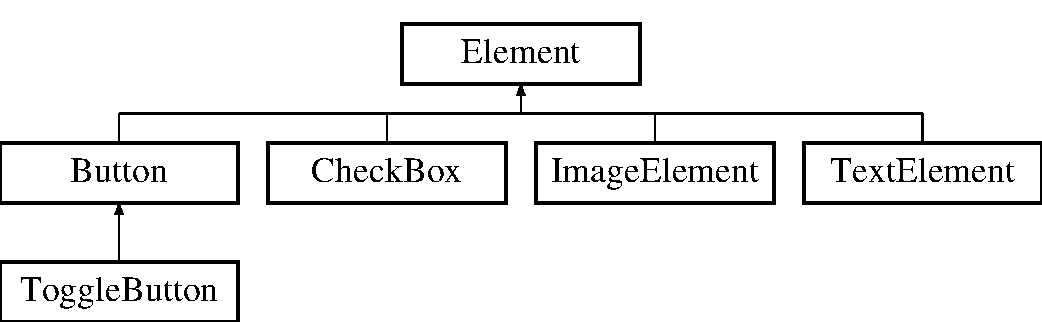
\includegraphics[height=3.000000cm]{class_element}
\end{center}
\end{figure}
\subsection*{Public Member Functions}
\begin{DoxyCompactItemize}
\item 
\hyperlink{class_element_ab0d0e20be9a36ae676202db753faeec9}{Element} ()
\begin{DoxyCompactList}\small\item\em Default Constructor. \end{DoxyCompactList}\item 
\hyperlink{class_element_ae385b104c66f092731777d70775b7f55}{Element} (int x, int y)
\item 
\hyperlink{class_element_aabaef3fcc0959ea3c5b43f59522d0a1e}{Element} (int x, int y, int xs, int ys)
\item 
virtual \hyperlink{class_element_a13d54ba9c08b6bec651402f1c2bb002c}{$\sim$\-Element} ()
\item 
virtual void \hyperlink{class_element_a5a35a40d6797bf8b6ebe1b76090244fd}{clear\-Result} ()
\item 
\hyperlink{class_image}{Image} $\ast$ \hyperlink{class_element_a2410f72a9b5abcf43641ef1b9e50f646}{render} ()
\item 
void \hyperlink{class_element_af3291346742556571a5c8578d2fc7026}{register\-Callback} (void($\ast$func)(void $\ast$))
\item 
void \hyperlink{class_element_aa1a3a8de669ecc840d2f2fb1e338300f}{mouse\-Input} (int x, int y)
\item 
void \hyperlink{class_element_a5e5de37f6b79a3a952d021ba15b3912d}{add\-Child} (\hyperlink{class_element}{Element} $\ast$child)
\item 
void \hyperlink{class_element_ae222484e55d330ddfd7869510b10ec09}{set\-X} (unsigned int x)
\item 
void \hyperlink{class_element_a95ea0342571b8521028b8321ba915227}{set\-Y} (unsigned int y)
\item 
void \hyperlink{class_element_aab1f2476247f365f6755dc2913d205b3}{set\-Z} (float z)
\item 
unsigned int \hyperlink{class_element_a4d41f5af2e3e5787945915a3b803131a}{get\-Id} ()
\item 
void \hyperlink{class_element_a185f979ca317ede0dd270c7940b2a0a2}{set\-Width} (unsigned int width)
\item 
void \hyperlink{class_element_aa3aaacaf56fb94deaa14f6b0d172ab65}{set\-Height} (unsigned int height)
\item 
void \hyperlink{class_element_aee4a1536e9e19eec9970522bb664550d}{set\-Dirty} (bool dirty)
\item 
bool \hyperlink{class_element_aa931ea96e0f488ffe00b7bef715ef24c}{operator$<$} (const \hyperlink{class_element}{Element} \&other)
\end{DoxyCompactItemize}
\subsection*{Protected Attributes}
\begin{DoxyCompactItemize}
\item 
unsigned int \hyperlink{class_element_a53e4a4ffd5e4e60ce40f55f910d11f23}{\-\_\-x\-Coord}
\item 
unsigned int \hyperlink{class_element_ab7215197a138c164d0ab07d7632e2ef2}{\-\_\-y\-Coord}
\item 
unsigned int \hyperlink{class_element_a559a2b7894e65668aee75346a3976f86}{\-\_\-width}
\item 
unsigned int \hyperlink{class_element_a6118137bfca71319ebaaa0d87be60cf3}{\-\_\-height}
\item 
\hyperlink{class_image}{Image} $\ast$ \hyperlink{class_element_ac79e1d8bac0f2b6d23f9ae156d4b6cce}{\-\_\-result}
\end{DoxyCompactItemize}


\subsection{Detailed Description}
The base class that all G\-U\-I elements derive from. 

This class provides a standard interface that is required for element traversal, rendering, and events. 

Definition at line 22 of file Element.\-h.



\subsection{Constructor \& Destructor Documentation}
\hypertarget{class_element_ab0d0e20be9a36ae676202db753faeec9}{\index{Element@{Element}!Element@{Element}}
\index{Element@{Element}!Element@{Element}}
\subsubsection[{Element}]{\setlength{\rightskip}{0pt plus 5cm}Element\-::\-Element (
\begin{DoxyParamCaption}
{}
\end{DoxyParamCaption}
)}}\label{class_element_ab0d0e20be9a36ae676202db753faeec9}


Default Constructor. 

Creates an element positioned at (0,0) with dimensions (0,0). 

Definition at line 10 of file Element.\-cpp.

\hypertarget{class_element_ae385b104c66f092731777d70775b7f55}{\index{Element@{Element}!Element@{Element}}
\index{Element@{Element}!Element@{Element}}
\subsubsection[{Element}]{\setlength{\rightskip}{0pt plus 5cm}Element\-::\-Element (
\begin{DoxyParamCaption}
\item[{int}]{x, }
\item[{int}]{y}
\end{DoxyParamCaption}
)}}\label{class_element_ae385b104c66f092731777d70775b7f55}
Creates an element positioned at (x,y) with dimensions (0,0). 

Definition at line 24 of file Element.\-cpp.

\hypertarget{class_element_aabaef3fcc0959ea3c5b43f59522d0a1e}{\index{Element@{Element}!Element@{Element}}
\index{Element@{Element}!Element@{Element}}
\subsubsection[{Element}]{\setlength{\rightskip}{0pt plus 5cm}Element\-::\-Element (
\begin{DoxyParamCaption}
\item[{int}]{x, }
\item[{int}]{y, }
\item[{int}]{xs, }
\item[{int}]{ys}
\end{DoxyParamCaption}
)}}\label{class_element_aabaef3fcc0959ea3c5b43f59522d0a1e}


Definition at line 39 of file Element.\-cpp.

\hypertarget{class_element_a13d54ba9c08b6bec651402f1c2bb002c}{\index{Element@{Element}!$\sim$\-Element@{$\sim$\-Element}}
\index{$\sim$\-Element@{$\sim$\-Element}!Element@{Element}}
\subsubsection[{$\sim$\-Element}]{\setlength{\rightskip}{0pt plus 5cm}Element\-::$\sim$\-Element (
\begin{DoxyParamCaption}
{}
\end{DoxyParamCaption}
)\hspace{0.3cm}{\ttfamily [virtual]}}}\label{class_element_a13d54ba9c08b6bec651402f1c2bb002c}


Definition at line 53 of file Element.\-cpp.



\subsection{Member Function Documentation}
\hypertarget{class_element_a5e5de37f6b79a3a952d021ba15b3912d}{\index{Element@{Element}!add\-Child@{add\-Child}}
\index{add\-Child@{add\-Child}!Element@{Element}}
\subsubsection[{add\-Child}]{\setlength{\rightskip}{0pt plus 5cm}void Element\-::add\-Child (
\begin{DoxyParamCaption}
\item[{{\bf Element} $\ast$}]{child}
\end{DoxyParamCaption}
)}}\label{class_element_a5e5de37f6b79a3a952d021ba15b3912d}


Definition at line 81 of file Element.\-cpp.

\hypertarget{class_element_a5a35a40d6797bf8b6ebe1b76090244fd}{\index{Element@{Element}!clear\-Result@{clear\-Result}}
\index{clear\-Result@{clear\-Result}!Element@{Element}}
\subsubsection[{clear\-Result}]{\setlength{\rightskip}{0pt plus 5cm}virtual void Element\-::clear\-Result (
\begin{DoxyParamCaption}
{}
\end{DoxyParamCaption}
)\hspace{0.3cm}{\ttfamily [inline]}, {\ttfamily [virtual]}}}\label{class_element_a5a35a40d6797bf8b6ebe1b76090244fd}


Reimplemented in \hyperlink{class_image_element_aa785ef26786dc59b0e66a71e465b3e31}{Image\-Element}, and \hyperlink{class_text_element_a2d61f3953226d9d4d06d4003d6c33c34}{Text\-Element}.



Definition at line 28 of file Element.\-h.

\hypertarget{class_element_a4d41f5af2e3e5787945915a3b803131a}{\index{Element@{Element}!get\-Id@{get\-Id}}
\index{get\-Id@{get\-Id}!Element@{Element}}
\subsubsection[{get\-Id}]{\setlength{\rightskip}{0pt plus 5cm}unsigned int Element\-::get\-Id (
\begin{DoxyParamCaption}
{}
\end{DoxyParamCaption}
)\hspace{0.3cm}{\ttfamily [inline]}}}\label{class_element_a4d41f5af2e3e5787945915a3b803131a}


Definition at line 39 of file Element.\-h.

\hypertarget{class_element_aa1a3a8de669ecc840d2f2fb1e338300f}{\index{Element@{Element}!mouse\-Input@{mouse\-Input}}
\index{mouse\-Input@{mouse\-Input}!Element@{Element}}
\subsubsection[{mouse\-Input}]{\setlength{\rightskip}{0pt plus 5cm}void Element\-::mouse\-Input (
\begin{DoxyParamCaption}
\item[{int}]{x, }
\item[{int}]{y}
\end{DoxyParamCaption}
)}}\label{class_element_aa1a3a8de669ecc840d2f2fb1e338300f}


Definition at line 62 of file Element.\-cpp.

\hypertarget{class_element_aa931ea96e0f488ffe00b7bef715ef24c}{\index{Element@{Element}!operator$<$@{operator$<$}}
\index{operator$<$@{operator$<$}!Element@{Element}}
\subsubsection[{operator$<$}]{\setlength{\rightskip}{0pt plus 5cm}bool Element\-::operator$<$ (
\begin{DoxyParamCaption}
\item[{const {\bf Element} \&}]{other}
\end{DoxyParamCaption}
)\hspace{0.3cm}{\ttfamily [inline]}}}\label{class_element_aa931ea96e0f488ffe00b7bef715ef24c}


Definition at line 44 of file Element.\-h.

\hypertarget{class_element_af3291346742556571a5c8578d2fc7026}{\index{Element@{Element}!register\-Callback@{register\-Callback}}
\index{register\-Callback@{register\-Callback}!Element@{Element}}
\subsubsection[{register\-Callback}]{\setlength{\rightskip}{0pt plus 5cm}void Element\-::register\-Callback (
\begin{DoxyParamCaption}
\item[{void($\ast$)(void $\ast$)}]{func}
\end{DoxyParamCaption}
)}}\label{class_element_af3291346742556571a5c8578d2fc7026}


Definition at line 76 of file Element.\-cpp.

\hypertarget{class_element_a2410f72a9b5abcf43641ef1b9e50f646}{\index{Element@{Element}!render@{render}}
\index{render@{render}!Element@{Element}}
\subsubsection[{render}]{\setlength{\rightskip}{0pt plus 5cm}{\bf Image} $\ast$ Element\-::render (
\begin{DoxyParamCaption}
{}
\end{DoxyParamCaption}
)}}\label{class_element_a2410f72a9b5abcf43641ef1b9e50f646}


Definition at line 91 of file Element.\-cpp.

\hypertarget{class_element_aee4a1536e9e19eec9970522bb664550d}{\index{Element@{Element}!set\-Dirty@{set\-Dirty}}
\index{set\-Dirty@{set\-Dirty}!Element@{Element}}
\subsubsection[{set\-Dirty}]{\setlength{\rightskip}{0pt plus 5cm}void Element\-::set\-Dirty (
\begin{DoxyParamCaption}
\item[{bool}]{dirty}
\end{DoxyParamCaption}
)\hspace{0.3cm}{\ttfamily [inline]}}}\label{class_element_aee4a1536e9e19eec9970522bb664550d}


Definition at line 42 of file Element.\-h.

\hypertarget{class_element_aa3aaacaf56fb94deaa14f6b0d172ab65}{\index{Element@{Element}!set\-Height@{set\-Height}}
\index{set\-Height@{set\-Height}!Element@{Element}}
\subsubsection[{set\-Height}]{\setlength{\rightskip}{0pt plus 5cm}void Element\-::set\-Height (
\begin{DoxyParamCaption}
\item[{unsigned int}]{height}
\end{DoxyParamCaption}
)\hspace{0.3cm}{\ttfamily [inline]}}}\label{class_element_aa3aaacaf56fb94deaa14f6b0d172ab65}


Definition at line 41 of file Element.\-h.

\hypertarget{class_element_a185f979ca317ede0dd270c7940b2a0a2}{\index{Element@{Element}!set\-Width@{set\-Width}}
\index{set\-Width@{set\-Width}!Element@{Element}}
\subsubsection[{set\-Width}]{\setlength{\rightskip}{0pt plus 5cm}void Element\-::set\-Width (
\begin{DoxyParamCaption}
\item[{unsigned int}]{width}
\end{DoxyParamCaption}
)\hspace{0.3cm}{\ttfamily [inline]}}}\label{class_element_a185f979ca317ede0dd270c7940b2a0a2}


Definition at line 40 of file Element.\-h.

\hypertarget{class_element_ae222484e55d330ddfd7869510b10ec09}{\index{Element@{Element}!set\-X@{set\-X}}
\index{set\-X@{set\-X}!Element@{Element}}
\subsubsection[{set\-X}]{\setlength{\rightskip}{0pt plus 5cm}void Element\-::set\-X (
\begin{DoxyParamCaption}
\item[{unsigned int}]{x}
\end{DoxyParamCaption}
)\hspace{0.3cm}{\ttfamily [inline]}}}\label{class_element_ae222484e55d330ddfd7869510b10ec09}


Definition at line 36 of file Element.\-h.

\hypertarget{class_element_a95ea0342571b8521028b8321ba915227}{\index{Element@{Element}!set\-Y@{set\-Y}}
\index{set\-Y@{set\-Y}!Element@{Element}}
\subsubsection[{set\-Y}]{\setlength{\rightskip}{0pt plus 5cm}void Element\-::set\-Y (
\begin{DoxyParamCaption}
\item[{unsigned int}]{y}
\end{DoxyParamCaption}
)\hspace{0.3cm}{\ttfamily [inline]}}}\label{class_element_a95ea0342571b8521028b8321ba915227}


Definition at line 37 of file Element.\-h.

\hypertarget{class_element_aab1f2476247f365f6755dc2913d205b3}{\index{Element@{Element}!set\-Z@{set\-Z}}
\index{set\-Z@{set\-Z}!Element@{Element}}
\subsubsection[{set\-Z}]{\setlength{\rightskip}{0pt plus 5cm}void Element\-::set\-Z (
\begin{DoxyParamCaption}
\item[{float}]{z}
\end{DoxyParamCaption}
)\hspace{0.3cm}{\ttfamily [inline]}}}\label{class_element_aab1f2476247f365f6755dc2913d205b3}


Definition at line 38 of file Element.\-h.



\subsection{Member Data Documentation}
\hypertarget{class_element_a6118137bfca71319ebaaa0d87be60cf3}{\index{Element@{Element}!\-\_\-height@{\-\_\-height}}
\index{\-\_\-height@{\-\_\-height}!Element@{Element}}
\subsubsection[{\-\_\-height}]{\setlength{\rightskip}{0pt plus 5cm}unsigned int Element\-::\-\_\-height\hspace{0.3cm}{\ttfamily [protected]}}}\label{class_element_a6118137bfca71319ebaaa0d87be60cf3}


Definition at line 50 of file Element.\-h.

\hypertarget{class_element_ac79e1d8bac0f2b6d23f9ae156d4b6cce}{\index{Element@{Element}!\-\_\-result@{\-\_\-result}}
\index{\-\_\-result@{\-\_\-result}!Element@{Element}}
\subsubsection[{\-\_\-result}]{\setlength{\rightskip}{0pt plus 5cm}{\bf Image}$\ast$ Element\-::\-\_\-result\hspace{0.3cm}{\ttfamily [protected]}}}\label{class_element_ac79e1d8bac0f2b6d23f9ae156d4b6cce}


Definition at line 51 of file Element.\-h.

\hypertarget{class_element_a559a2b7894e65668aee75346a3976f86}{\index{Element@{Element}!\-\_\-width@{\-\_\-width}}
\index{\-\_\-width@{\-\_\-width}!Element@{Element}}
\subsubsection[{\-\_\-width}]{\setlength{\rightskip}{0pt plus 5cm}unsigned int Element\-::\-\_\-width\hspace{0.3cm}{\ttfamily [protected]}}}\label{class_element_a559a2b7894e65668aee75346a3976f86}


Definition at line 49 of file Element.\-h.

\hypertarget{class_element_a53e4a4ffd5e4e60ce40f55f910d11f23}{\index{Element@{Element}!\-\_\-x\-Coord@{\-\_\-x\-Coord}}
\index{\-\_\-x\-Coord@{\-\_\-x\-Coord}!Element@{Element}}
\subsubsection[{\-\_\-x\-Coord}]{\setlength{\rightskip}{0pt plus 5cm}unsigned int Element\-::\-\_\-x\-Coord\hspace{0.3cm}{\ttfamily [protected]}}}\label{class_element_a53e4a4ffd5e4e60ce40f55f910d11f23}


Definition at line 47 of file Element.\-h.

\hypertarget{class_element_ab7215197a138c164d0ab07d7632e2ef2}{\index{Element@{Element}!\-\_\-y\-Coord@{\-\_\-y\-Coord}}
\index{\-\_\-y\-Coord@{\-\_\-y\-Coord}!Element@{Element}}
\subsubsection[{\-\_\-y\-Coord}]{\setlength{\rightskip}{0pt plus 5cm}unsigned int Element\-::\-\_\-y\-Coord\hspace{0.3cm}{\ttfamily [protected]}}}\label{class_element_ab7215197a138c164d0ab07d7632e2ef2}


Definition at line 48 of file Element.\-h.



The documentation for this class was generated from the following files\-:\begin{DoxyCompactItemize}
\item 
element/\hyperlink{_element_8h}{Element.\-h}\item 
element/\hyperlink{_element_8cpp}{Element.\-cpp}\end{DoxyCompactItemize}

\chapter{File Documentation}
\hypertarget{_element_8cpp}{\section{element/\-Element.cpp File Reference}
\label{_element_8cpp}\index{element/\-Element.\-cpp@{element/\-Element.\-cpp}}
}
{\ttfamily \#include \char`\"{}Element.\-h\char`\"{}}\\*
{\ttfamily \#include $<$iostream$>$}\\*
{\ttfamily \#include $<$algorithm$>$}\\*
{\ttfamily \#include $<$stdio.\-h$>$}\\*
{\ttfamily \#include \char`\"{}../image/\-Image.\-h\char`\"{}}\\*

\hypertarget{_element_8h}{\section{element/\-Element.h File Reference}
\label{_element_8h}\index{element/\-Element.\-h@{element/\-Element.\-h}}
}
{\ttfamily \#include $<$vector$>$}\\*
{\ttfamily \#include $<$algorithm$>$}\\*
{\ttfamily \#include \char`\"{}../image/\-Image.\-h\char`\"{}}\\*
\subsection*{Classes}
\begin{DoxyCompactItemize}
\item 
class \hyperlink{class_element}{Element}
\begin{DoxyCompactList}\small\item\em The base class that all G\-U\-I elements derive from. \end{DoxyCompactList}\end{DoxyCompactItemize}


\subsection{Detailed Description}
This file contains the \hyperlink{class_element}{Element} class. 

Definition in file \hyperlink{_element_8h_source}{Element.\-h}.


\hypertarget{_main_8cpp}{\section{Main.\-cpp File Reference}
\label{_main_8cpp}\index{Main.\-cpp@{Main.\-cpp}}
}
{\ttfamily \#include $<$iostream$>$}\\*
{\ttfamily \#include $<$vector$>$}\\*
{\ttfamily \#include \char`\"{}Element.\-h\char`\"{}}\\*
\subsection*{Functions}
\begin{DoxyCompactItemize}
\item 
int \hyperlink{_main_8cpp_ae66f6b31b5ad750f1fe042a706a4e3d4}{main} ()
\end{DoxyCompactItemize}


\subsection{Function Documentation}
\hypertarget{_main_8cpp_ae66f6b31b5ad750f1fe042a706a4e3d4}{\index{Main.\-cpp@{Main.\-cpp}!main@{main}}
\index{main@{main}!Main.cpp@{Main.\-cpp}}
\subsubsection[{main}]{\setlength{\rightskip}{0pt plus 5cm}int main (
\begin{DoxyParamCaption}
{}
\end{DoxyParamCaption}
)}}\label{_main_8cpp_ae66f6b31b5ad750f1fe042a706a4e3d4}


Definition at line 6 of file Main.\-cpp.


\addcontentsline{toc}{part}{Index}
\printindex
\end{document}
